%---------------------------------------------------------------
\chapter{Feedback Usage}
%---------------------------------------------------------------

\begin{chapterabstract}
	After observing that the feedback vector can be polluted with information, the next step is the understanding of how the feedback is used in the compilation. Ultimately, we want to categorize slots in how they are used, and quantify how much of the recorded information influences the compilation, as well as identifying the reason for why slot was not used in a compilation. First, we define the categories of how a slot can be used or not used. Next we analyze the usage of feedback in Ř. Lastly, we acknowledge the limitations of the analysis and discus alternative approaches.
\end{chapterabstract}

In this chapter, we only focus on the \textit{type slots} because, as observed in the feedback pollution analysis, these suffer from pollution the most. They are also the most variable parts, and having a much larger state space they allow for a richer analysis.

%---------------------------------------------------------------
\section{Definitions}
%---------------------------------------------------------------

\begin{itemize}
	\item{} We define a \textit{non-empty slot} as a slot that has at least one observation. An \textit{empty} slot means that the instruction was never executed.
	\item{} We say that a slot is \textit{referenced} if it is part of a function that is compiled to native, including slots inside inlined functions.
	\item{} A slot is then \textit{read} if during a compilation the information in the slot is observed.
	\item{} A \textit{used slot} is a type feedback slot that has an assumption connected with it in the final version of PIR (after all optimizations finished running). A used slot is always non-empty.
\end{itemize}

%---------------------------------------------------------------
\subsubsection*{Used Slots}
%---------------------------------------------------------------

When an assumption on a type is emited, it has a structure outlined in listing \ref{lst:assume-structure}. The value we speculate on is in the register \texttt{\%1} with a \textit{static type}, which is inferred from the call context, known types of builtins, and preceding assumptions. The instruction has also an associated \textit{feedback type}, which is the union of all types observed in the interpreter. The speculated value is an input to an \texttt{IsType} instruction, which checks the actual runtime type against the \textit{assumed type}. The result of the type check is then an input to the \texttt{Assume} instruction, along with the corresponding \texttt{Checkpoint}, resulting in a deoptimization if the type check fails.

\begin{listing}[H]
	\centering
	\begin{minted}[linenos=false]{\pirlexer}
[static type]   %1 = [instruction]   args... <feedback type>
lgl$#-          %2 = IsType          %1 isA [assumed type]
void                 Assume          %2, [checkpoint]
  \end{minted}
	\caption{PIR code structure of type assumption}\label{lst:assume-structure}
\end{listing}

The construction of the assumed type is not as straight-forward as it might seem. We illustrate the process in figure \ref{fig:types-venn}, where larger area means a more general type.

\begin{figure}
	\centering
	\includediagram{8}
	\caption{Illustration of the relationship between static, feedback, expected and assumed types}\label{fig:types-venn}
\end{figure}

First, we construct an \textit{expected type} by intersecting the static and feedback type. If this intersection is empty, no assumption is emited, otherwise we procede to create the assumed type.

It can happen that the static type is more precise than the feedback type (in the figure \ref{fig:types-venn}, the green area is non-empty). We call this a \textit{narrowing} of the feedback type, as the static type narrows the feedback information into a more specific one. For example, this happens when we statically know that the value we are speculating on is a scalar, but we have observed also non-scalar values.

If the R type of the expected type is not integer, float or logical vector, we do not speculate on it as it is. The optimizations are not able to use this precise of an information, thus the compiler tries to relax the assumption first. We call this \textit{widening}, as we are widening the information of the feedback type (and also the expected type), while still staying in the bounds of the static type. This results in the final assumed type. If we cannot reasonably relax the type, we give up on assuming. A type can be both widened and narrowed at the same time.

If the assumed type is equal to the feedback type, we say that the feedback was used as \textit{exact match}. This implies that it has not been narrowed, nor widened.

%---------------------------------------------------------------
\subsubsection*{Unused Slots}
%---------------------------------------------------------------

For the unused slots, we want to understand what is the reason why they are not used and how does this play with the slot being polluted. We consider only non-empty slots, as empty type feedback slot cannot be speculated on.

The first reason we have identified is that the \textit{slot is optimized away}. This happens when the instruction the type feedback is attached to is not present in the final optimized PIR code. There are many reason for removing instruction during optimizations, but the most common ones are \textit{constant folding} and \textit{dead code elimination}.

Another reason for not using a slot is because it contains \textit{redundant information}. Formally we say that an \textit{unused slot is redundant} if its type information is equivalent to any other slot, both used or unused. This might be a broad definition, but it can still reveal to us data about the slot usage.

Note that reduntant slots and slots that are optimized away are not disjunct categories.

There are more reasons to why a slot might not be used, like the information in the feedback is not useful for speculation, or the information is overriden by static information. We do not categorize these further, as this would require a much deeper analysis, possibly needing a rewrite of parts of the compiler in order to observe.

%---------------------------------------------------------------
\subsubsection*{Polymorphic Slots}
%---------------------------------------------------------------

A \textit{polymorphic slot} is slot that has observed more than one distinct type. This is a superset of the \textit{polluted slots}, i.e. a polluted slot is always polymorphic, but a polymorphic slot is not always polluted. A non-polymorphic slot is \textit{monomorphic}.

Observing polymorphic slots allows us to outline the usage of polluted slots, while also observing the behaviour of slots that have (potentially) too general of an information even before the first compilation.

%---------------------------------------------------------------
\section{Methodology}
%---------------------------------------------------------------

In order to collect all the information needed, we had to directly instrument the Ř compiler. We inspect the PIR code of closures and collect information about all of the assumptions, including the corresponding type test and cast instructions. We use the rich Ř APIs for traversing code and inspecting instructions. All of the code for collecting data is in the main repository in the branch \texttt{feedback-in-jits}\footnote{\url{https://github.com/reactorlabs/rir/tree/feedback-in-jits}}.

Our unit for collecting information is a \textit{closure version compilation}, one lowering of a closure from PIR to native code. For each compilation, we define its \textit{universe} as the compiled closure and all of its inlinees. All counts are then in reference to this universe, so for example the number of referenced slot of one compilation is the sum of all slots in the universe. We ignore multiple inlinings of the same closure in one compilation as we have observed that in most cases the slots are used in the same way across all inlinings.

The final data is aggregated over these closure version compilations. Thus when we say that there were two used slots, we mean that over all compilations a slot was used two times, it might even be the same slot. The reason for this was that between the individual compilations, the state of the slots can change, and there is no reasonable way to reference and quantify all slots after the program terminates.

\begin{table}[t]
	\makebox[\linewidth]{%
		\begin{tabular}{l l l l l}
			\hline
			\textbf{Program name}   & \textbf{Benchmark suite} & \textbf{Lines of code} & \textbf{Compilations} & \textbf{Referenced slots} \\
			\hline
			bounce\_nonames\_simple & Are We Fast Yet          & 58                     & 11                    & 264                       \\
			mandelbrot              & Are We Fast Yet          & 65                     & 14                    & 358                       \\
			flexclust\_no\_s4       & Real Thing               & 163                    & 144                   & 5335                      \\
			volcano                 & Real Thing               & 63                     & 23                    & 2037                      \\
			binarytrees\_naive      & Shootout                 & 31                     & 22                    & 1070                      \\
			fannkuchredux           & Shootout                 & 63                     & 6                     & 251                       \\
			fannkuchredux\_naive    & Shootout                 & 62                     & 5                     & 244                       \\
			fasta\_naive\_2         & Shootout                 & 88                     & 17                    & 598                       \\
			knucleotide             & Shootout                 & 72                     & 59                    & 1493                      \\
			pidigits/pidigits       & Shootout                 & 333                    & 92                    & 5651                      \\
			titanic                 & -                        & 108                    & 2020                  & 66119                     \\
			\hline
		\end{tabular}
	}
	\caption{Overview of analyzed programs}\label{tbl:analysis-overview}
\end{table}

We ran the analysis on a selection of ten benchmarks from the Ř benchmark suite and the Titanic Kaggle notebook, outlined in table \ref{tbl:analysis-overview}. We can see that the Kaggle notebook has more compilations by an order of magnitude when compared to the benchmarks and thus also many more referenced slots. All of the experiments were ran with the invocation threshold for native compilation set to 10, as this allowed us to observe more compilations, while still preserving the characteristics.

%---------------------------------------------------------------
\section{Observations}
%---------------------------------------------------------------

\todo{correct numbers}

In constrast to the pollution analysis, while categorizing the slots we have observed that the Kaggle script behaves very much in the same way as the benchmark programs do. This is interesting, because they are written in very different ways and are doing different kinds of computations. This might point to a deeper issue connected with the behavior the Ř compiler.

\begin{figure}[t]
	\centering
	\begin{adjustwidth}{-3cm}{-3cm}
		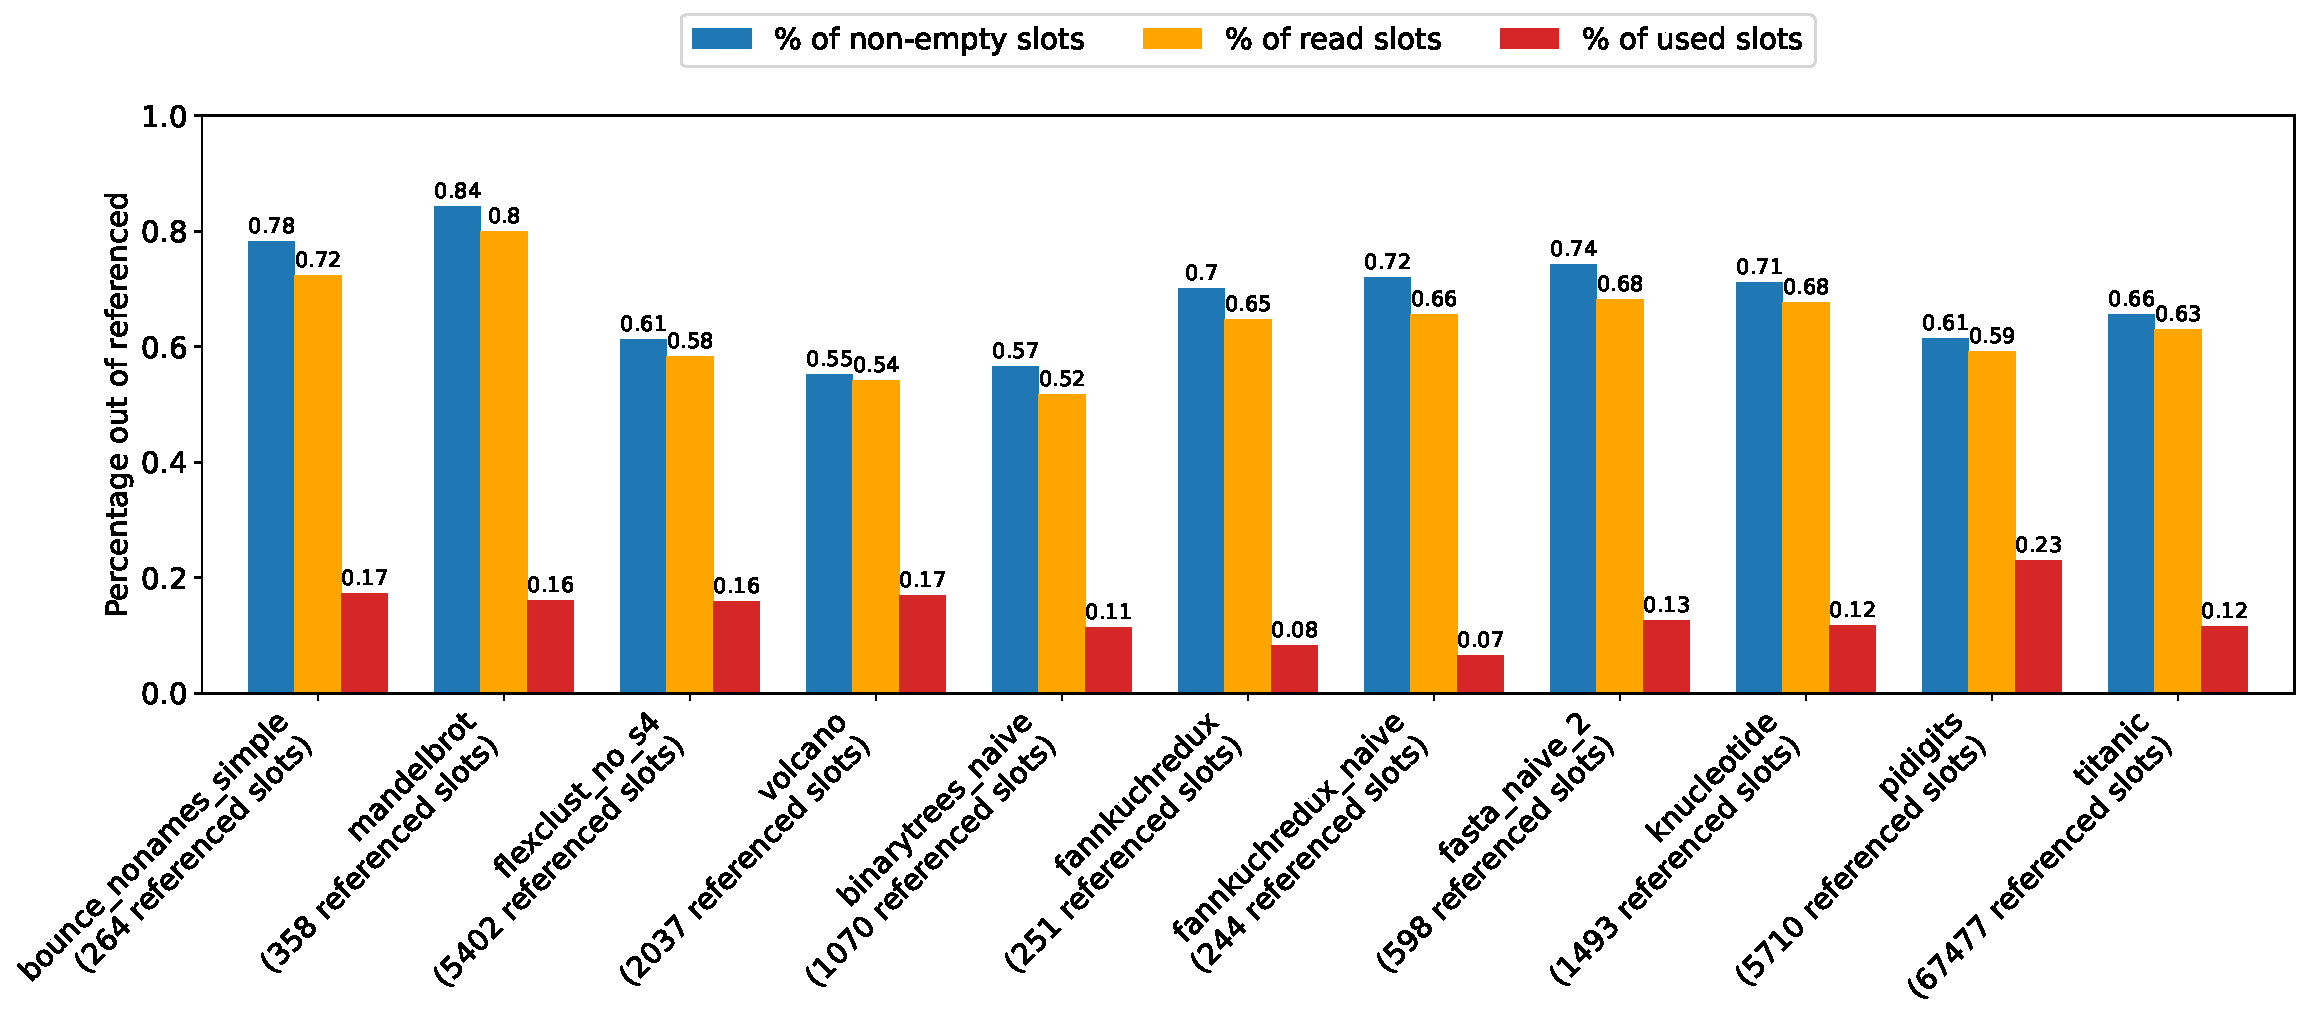
\includegraphics[width=1.5\textwidth]{figures/usage_overall.pdf}
	\end{adjustwidth}
	\caption{Usage of slots across closure compilations}\label{fig:graph-overview}
\end{figure}

In figure \ref{fig:graph-overview} is the categorization of used slots. We can see that most of the slots are not empty (68\% on average) and most of the non-empty slots are read (81\% on average), thus are considered for speculation. But on average only 14\% of slots are used (21\% of non-empty slots). This is surprising, as the recording of information is impacting the speed the bytecode interpreter, and yet the recorded information is used quite sparsely.

A hypothesis we had was that a polymorphic slot is less likely to be used. Out of the polymorphic slots, 25\% of them are used, compared to the non-empty monomorphic slots where 21\% are used. However, it is probably due to the fact that by their nature, polymorphic slots are on the paths of the program which are executed, thus there are less reasons to not use them \todo{reword}.

\begin{figure}[t]
	\centering
	\begin{adjustwidth}{-3cm}{-3cm}
		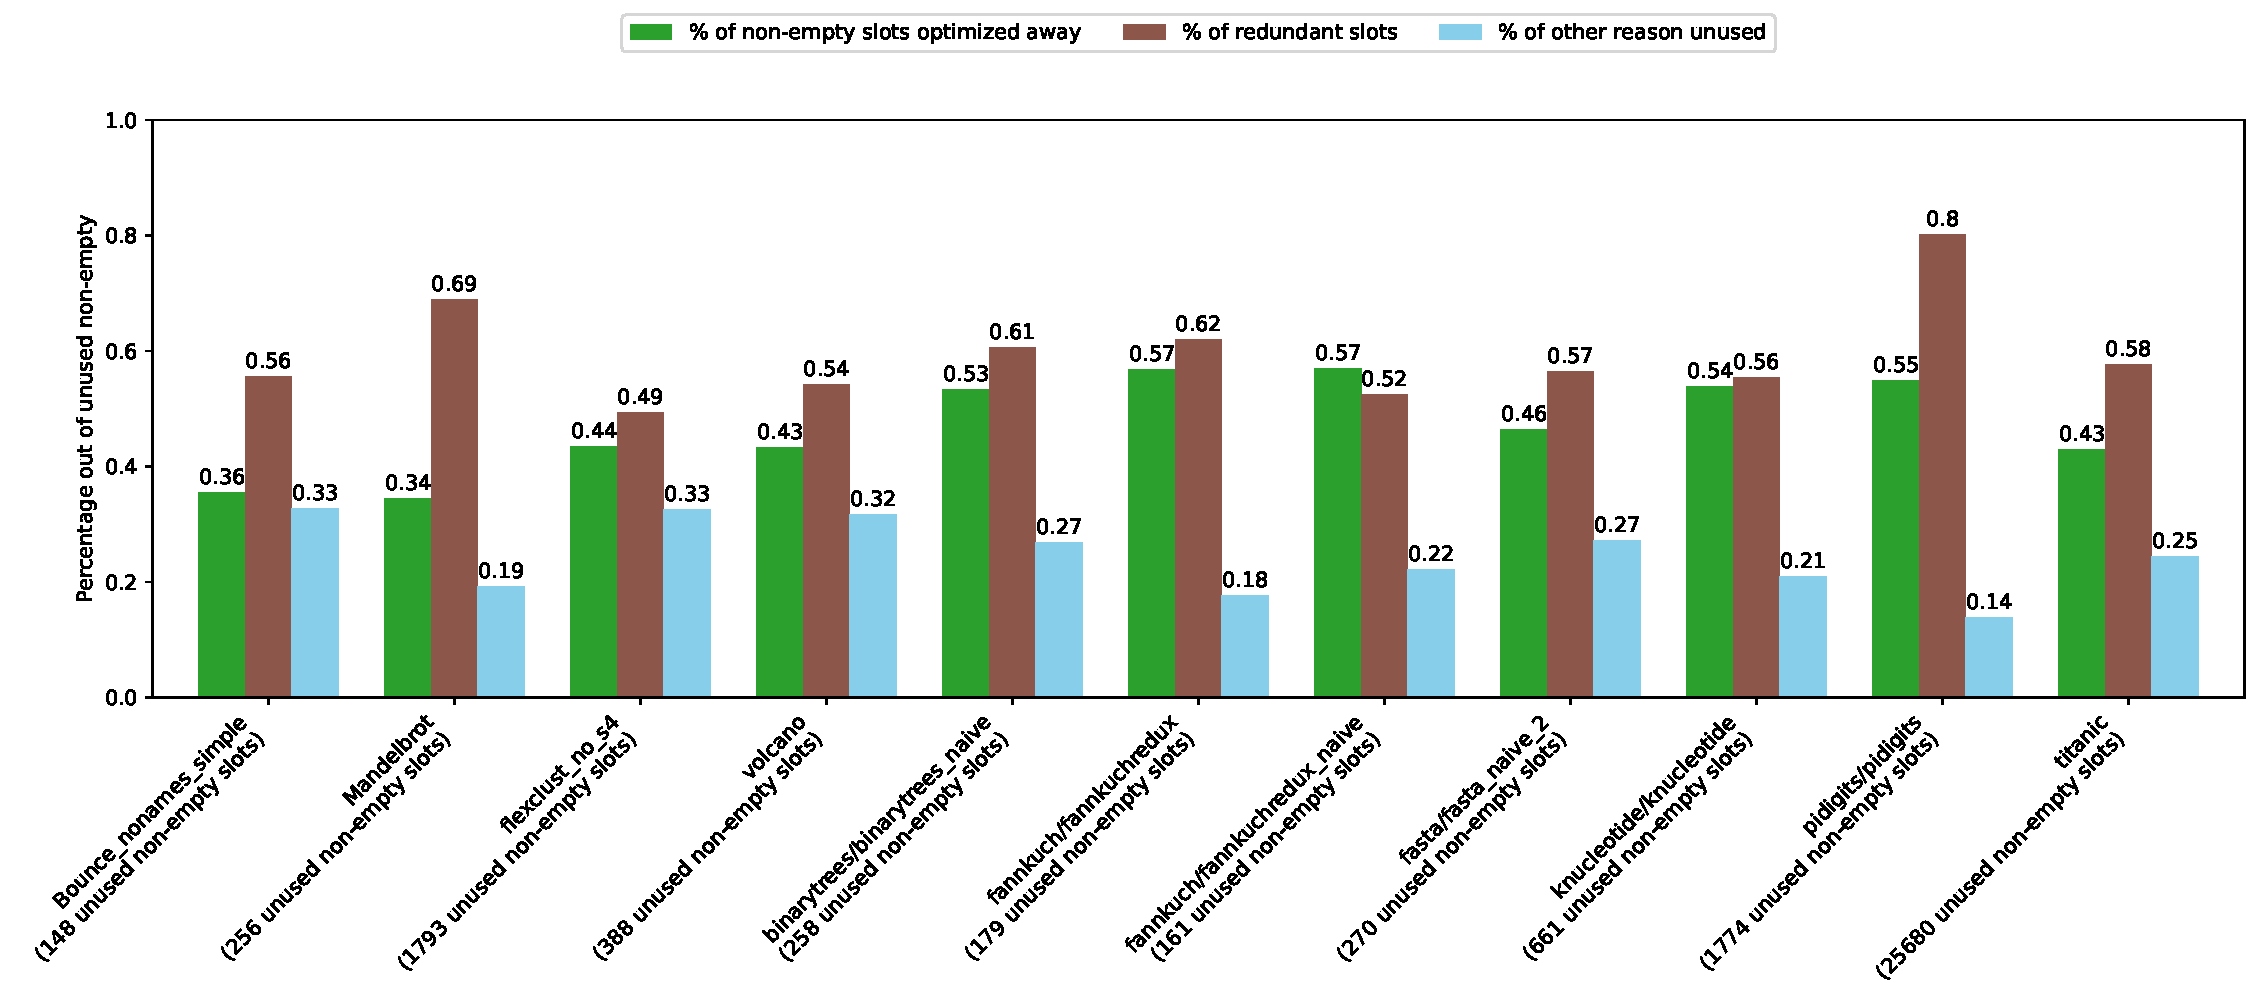
\includegraphics[width=1.5\textwidth]{figures/unused.pdf}
	\end{adjustwidth}
	\caption{Categorization of unused slots across closure compilations}\label{fig:graph-unused}
\end{figure}

When we consider the non-empty unused slots shown in figure \ref{fig:graph-unused}, we can see that the dominating cause for a slot not being used is redundancy, on average 59\% of all non-empty unsed slots. This is expected in the benchmarks because they usually only use one numeric type across the whole program. But the Kaggle script uses a lot of different types, yet 58\% of the unused slots are deemed redundant, which even is lower than the average. This leads us to believe that there is a deeper cause for a redundant slot in the way the information is collected in the interpreter, leaving a room for optimizations.

Observing the slots that are optimized away, they take on average 31\% of the non-empty unused slots. Separating the monomorphic and polymorphic slots, we see that 33\% of unused monomorphic slots are optimized aways, whereas only 26\% of unused polymorphic are optimized away. This might come from the same reasons as the comparison between monomorphic and polymorphic used slots, where the polymorphic ones are more likely to be on more frequently executed paths.

28\% of all slots are neither redundant nor optimized away. This might include some actually redundant slots that are not caught by our approximate analysis, but there might also be other reasons for not using a slot and these will probably overlap with the identified reasons. These need to be further analyzed.

\begin{figure}[t]
	\centering
	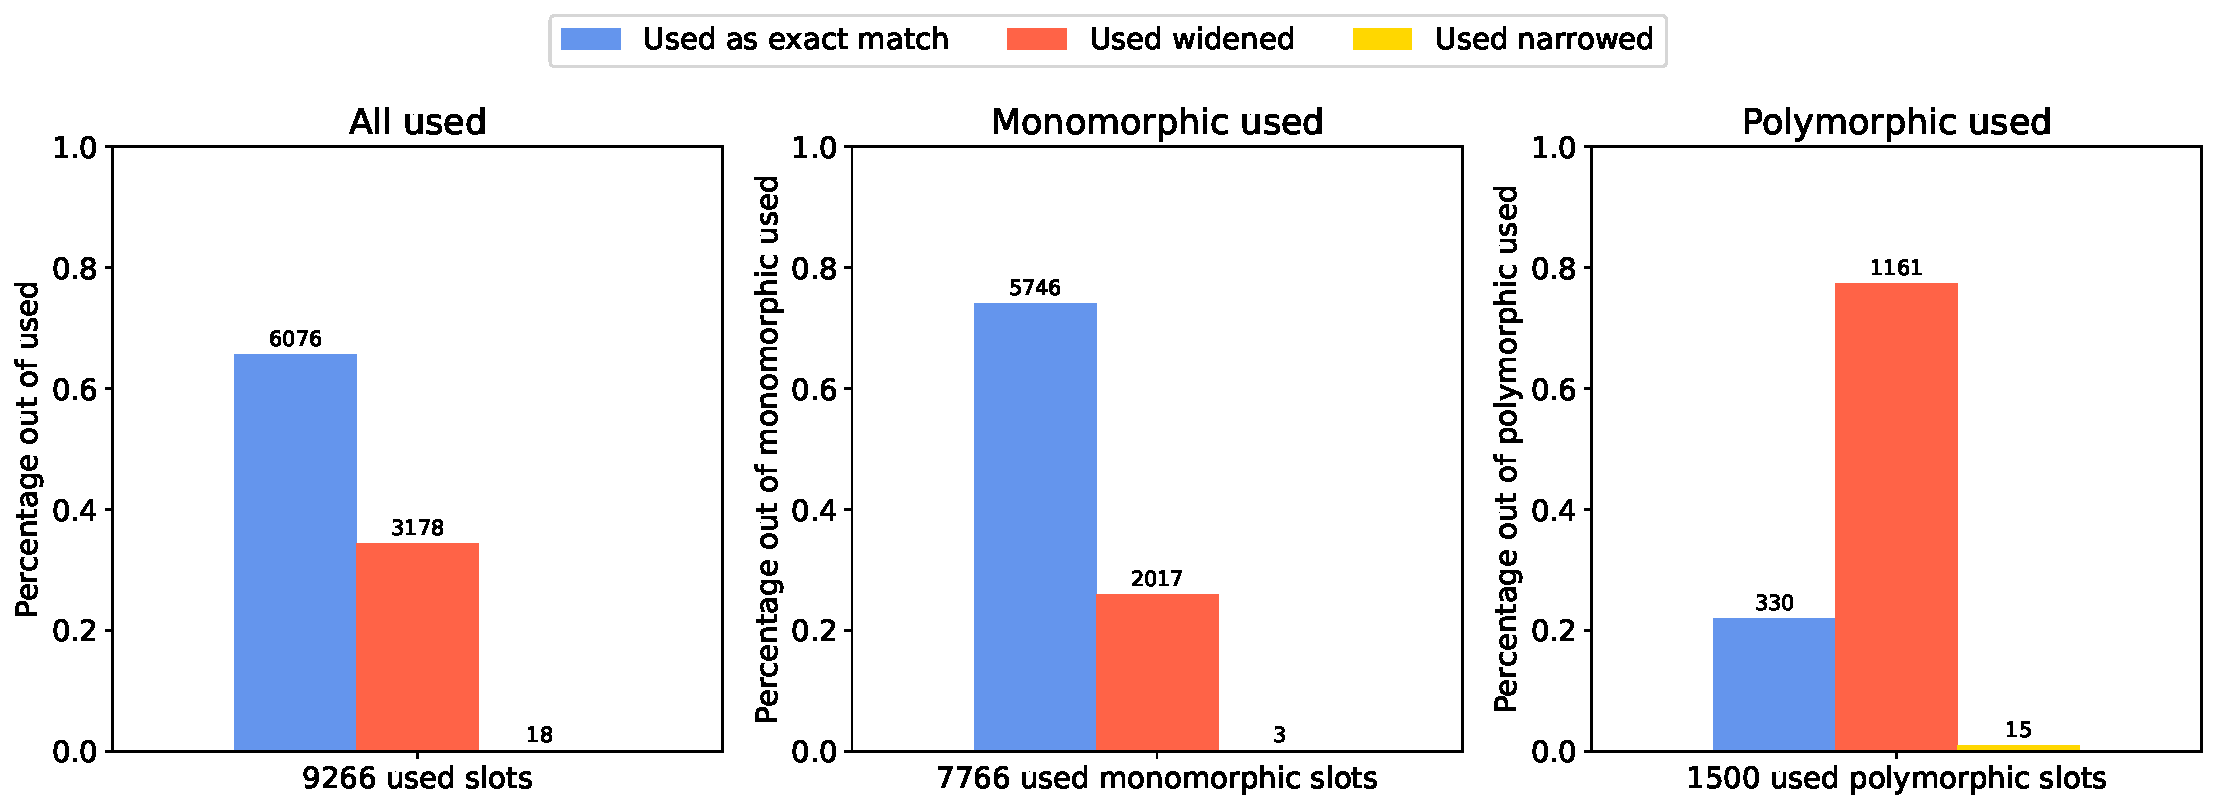
\includegraphics[width=\textwidth]{figures/used_all.pdf}
	\caption{Categorization of used slots}\label{fig:graph-used}
\end{figure}

When we look on the graph \ref{fig:graph-used}, we can see that more than half of the slots are used as exact match. If we split the monomorphic and polymorphic used slots, we can see an even bigger distinction. 81\% of used monomorphic slots are used as exact match, meaning that most of the time when a slot is not polymorphic it contains an information precise enough to be used as it is. On the other hand, 93\% of used polymorphic slots are widened. This is to be expected, as the polymorphic slots have a more general type that gets widened before an assumption is made.

For the polymorphic slots used as exact match, the feedback type is either a single non-scalar R type (integer, real or logical), or any R type which might be missing. In either case, the type is always not scalar and we have observed that it is not an object or even that it does not have any attributes. The polymorphism in these cases probably come from observing both scalar and non-scalar types. \todo{rewrite}

Interestingly, there are very few slots that are narrowed by the static information, 18 to be precise.

\begin{itemize}
	\item{} 2 of them have added information about the type not being NA. Since we do not record this information\footnote{In order to observe that a vector is not NA, we would need to inspect all elements of it and this is very costly for large vectors}, it is trivial for the static type to narrow it in this way. These are the only monomorphic slots that are narrowed.
	\item{} 4 slots are narrowed into a scalar type. This is due to the slot observing also non-scalar types, but the static type can specialize the observation.
	\item{} 2 slots have their type narrowed to a double and the only information used from the slot is that the value does not have attributes.
	\item{} In 9 cases, the static type removes a \enquote{might be missing} flag from the feedback type. In these cases we have observed too many values and the type feedback falls back to the most generic type, which has the flag that it might be a missing value. But this speculation is on a \texttt{Force} instruction, which when forcing a value that is missing result in an error, thus the result of \texttt{Force} is always not missing or it diverges.
\end{itemize}

%---------------------------------------------------------------
\subsubsection*{Conclusion}
%---------------------------------------------------------------

The main takeaway of the analysis is that a very low number of feedback slots is being used by the compiler. This leads to a time spent in the interpreter by recording observations being wasted. If we are able to detect which slots are truly redundant, we could optimize

Another key point is that a polymorphism, and by extend pollution, does not impact \textit{if} a slot is used in compilation, but it influences \textit{how} the feedback is used. Since the information in a polymorphic slot is more generic, we observe that it has to be widened before it is used.

Finally, in our experiments we see that the leading cause for a slot not being used is because it is reduntant. This leads us to belive there is room for improvement in the way the information gets recorded.

The analysis is freely available online on GitHub \footnote{\url{https://github.com/rihafilip/masters-thesis-analysis}}.

%---------------------------------------------------------------
\section{Limitations}
%---------------------------------------------------------------

The biggest obstacle we have encountered during the analysis is unknown origin of type information. Due to the architecture of the compiler, we are unable to precisely track how a type is constructed or how a type information is propagated. This leads to the broad definition of redundant slots, which might catch unrelated slots or miss dependent slots recording different information due to type coercions, as well as less precise analysis of the slots usage. Still, the presented results give us idea about the behaviour of individual type feedback slots.

Another drawback is the tracking of inlined functions. It is not uncommon that a function is inlined more than once in a single closure compilation, and this proves to be difficult to summarize without skewing the resulting numbers, as one slot might be used differently or used in one case and not used in the other. This might lead to double counts of a slot in multiple categories or missing a usage pattern, and we are aware of that \todo{rewrite the last part of sentence}.

While running the experiments, we have observed multiple runs of some of the benchmarks (namely flexclust\_no\_s4 and pidigits) and the Kaggle script result in different resulting numbers. However, the final characteristics are the same and the trends do not change. Therefore the numbers presented in this chapter are from a single run of the experiments.

